\documentclass[12pt]{article}
\usepackage[utf8]{inputenc}
\usepackage{amsmath,amssymb,hyperref,array,xcolor,multicol,verbatim,mathpazo,algorithm,algpseudocode,enumerate,tikz}
\usepackage[normalem]{ulem}
\usepackage{graphicx}

\newenvironment{problem}[2][Problem]{\begin{trivlist}
\item[\hskip \labelsep {\bfseries #1}\hskip \labelsep {\bfseries #2.}]}{\end{trivlist}}

\begin{document}

%%%% In most cases you won't need to edit anything above this line %%%%

\title{\vspace{-4cm}CS 270 Homework 4}
\author{Neel Gupta} 
\maketitle

\begin{problem}{1}
    Design a data structure that has the following properties. Assume $n$ elements in the structure and that the data structure property needs to be preserved at the end of each operation.
    \begin{itemize}
        \item Find median takes $O(1)$ time
        \item Insert takes $O(\log n)$ time
    \end{itemize}
    Do the following:
    \begin{enumerate}[(a)]
        \item Describe how your data structure will work.
        \item Give algorithms that implement Find-Median() and Insert() functions.
    \end{enumerate}
\end{problem}
\textit{Answer:} \\
(a) Consider using two heaps where one is a max-heap and the other is a min-heap. We can store the of the numbers greater than the current median in a min-heap and the numbers less than the current median in a max-heap. When the number of elements within the heaps differs by greater than 1, we will pop from the larger one to the smaller one until the number of elements in each heap differs by at most 1. At the beginning, we will add the first element to either the min or max heap arbitrarily, and we will store the current median and set it to this value. To add more elements, we will check whether the new number we are adding is less than or greater than the current median, and if it is greater, it will go in the min-heap, and if it is less than, it will go in the max-heap. If the number of elements in the heaps differ by only 1, we will update the current median to that value, else if the number of elements in the min-heap and max-heap are the same, then we will pop elements from both and take the average of them, which takes $O(1)$ in all cases. To add new elements, it is a comparision then addition into a max or min heap of size $\frac{n}{2}$ which takes $\log(n)$ time\\
\newpage
(b) \begin{algorithmic}
    \State Initialize min-heap $n$ and max-heap $x$ as empty 
    \State currentMedian $\gets null$
    \Procedure{Find-Median}{}
        \If{len($n$) == len($x$)}
            \State currentMedian $\gets \frac{(n.\text{pop}*x.\text{pop})}{2}$
        \ElsIf{$n$ is bigger than $x$}
            \State currentMedian $\gets n$.pop
        \ElsIf{$x$ is bigger than $n$}
            \State currentMedian $\gets x$.pop
        \EndIf
    \EndProcedure
    \Procedure{Insert}{val}
        \If{both $n$ and $x$ are empty}
            \State $n$.insert(val)
        \ElsIf{val $\leq$ currentMedian}
            \State $x$.insert(val)
        \Else
            \State $n$.insert(val)
        \EndIf
        \While{$|$len($n$)-len($x$)$|\geq 2$}
            \State pop elements from larger heap and add them to smaller heap
        \EndWhile
    \EndProcedure
\end{algorithmic}

\begin{problem}{2}
    Let us say that a graph $G=(V,E)$ is a near tree if it is connected and has at most $n+k$ edges, where $n=|V|$ and $k$ is a \textbf{constant}. Give an algorithm with running time $O(n)$ that takes a near tree $G$ with costs on its edges, and returns a minimum spanning tree of $G$. You may assume all edge costs are distinct.
\end{problem}
\textit{Answer:}
After applying the Cycle Property $k+1$ times, we are given an MST with $n-1$ edges. After preforming BFS $k+1$ times to find a cycle, we can delete the heaviest edge $e$ that causes this cycle. Through doing this reverse-delete type MST algorithm, we have deleted the heaviest edge in this cycle while maintaining the connectedness of the graph. If we do this $k+1$ times, we will have a new connected graph $H$ with $n-1$ edges which is the same as the MST of $G$. Since $H$ is a tree by the fact that it is connected and has $n-1$ nodes without any cycles, it is also in fact the minimum spanning tree. Let $m:=|E|$ and $n:=|V|$, then $n-1 \leq m \leq n+k$ by connectedness and near-tree property. The runtime of BFS is $O(m+n)$, but $m$ is a constant for a near-tree, so the runtime of BFS os $O(n)$. Finding the heaviest edge takes $O(n)$ time, so we have to find the heaviest edge $k+1$ times. Therefore the runtime of this algorithm is $O((k+1)n) = O(n)$.
\begin{problem}{3}
    A new startup FastRoute wants to route information along a path in a communication netweork, represented as a graph. Each vertex and edge represents a router and a wire between routers respectively. The wires are weighted by the maximum bandwidth they can support. FastRoute comes to you and asks you to develop al algorithm to find the path with maximum bandwidth from any source $s$ to any destination $t$. As you would expect, the bandwidth of a path is the minimum of the bandwidths of the edges on that path; the minimum edge is the bottleneck. Explain how to modify Dijkstra's algorithm to do this.
\end{problem}
\textit{Answer:}
\begin{itemize}
    \item Instead of having a distance array, we would have a capacity array which keeps the maximum-minimum capacity that is possible up that point. 
    \item In Dijkstra's, the first node is initialized as having 0 distance to itself and the rest are infinitely far in distance. In this modification, the source node has infinite capacity while each node in the graph that isn't in the source node has minimum (negative infinity) capacity because only edges have weights.
    \item We initialize a max-heap to store edge capacities, and at each iteration, we get the max capacity node and check whether we can get to a neighbor of the current edge in a larger capacity by going through the current node. If the capacity is higher between how we previously got to the current node and this new method of getting to that node, then we can update the new capacity and store the previous node which has now changed.
    \item At the beginning of each iteration, we can check whether we have found $-\infty$. If we have found it, then we can traverse backwards using our 
\end{itemize}
\begin{algorithmic}
    \Procedure{modifiedDijkstra}{G, start, end}
        \State Initialize capacity list of size $|V|$
        \State Initialize prev list of size $|V|$
        \State Initialize max-heap $Q$
        \State capacity $\gets -\infty$ 
        \State capacity[start] $\gets \infty$
        \State $Q \gets $ all vertices in $G$
        \While{$Q$ is not empty}
            \State currentNode $\gets Q$.pop
            \If{capacity[currentNode]=$-\infty$}
                \State break;
            \EndIf
            \For{each neighbor $n$ of currentNode}
                \State edgeCapacity $\gets$ capacity between currentNode and $n$
                \If {max(capacity[$n$], edgeCapacity) $>$ capacity[$n$]}
                    \State capacity[$n$] $\gets$ max(capacity[$n$], edgeCapacity)
                    \State prev[$n$] $\gets$ currentNode
                    \State $Q$.updateCapacity($n$)
                \EndIf
            \EndFor
        \EndWhile
        \State $u\gets $ end
        \While{$u\ne null$}
            \State path.add($u$)
            \State $u\gets $ prev[$u$]
        \EndWhile
        \State return reverse(path)
    \EndProcedure
\end{algorithmic}
\begin{problem}{4}
    Given a connected graph $G=(V,E)$ with positive edge weights. In $V$, $s$ and $t$ are two nodes for shortest path computation, prove or disprove with explanatations.
    \begin{enumerate}[(a)]
        \item If all edge weights are unique, then there is a single shortest path between any two nodes in $V$.
        \item If each edge's weight is increased by $k$, the shortest path cost between $s$ and $t$ will increase by a multiple of $k$.
        \item If the weight of some edge $e$ decreases by $k$, then the shortest path cost between $s$ and $t$ will decrease by at most $k$.
        \item If each edge's weight is replaced by its square, i.e. $w$ to $w^2$, then the shortest path between $s$ and $t$ will be the same as before but with different costs.
    \end{enumerate}
\end{problem}
\textit{Answer:}

(a) Consider the following graph where edge weights are unique and there are multiple shortest path distances from $s$ to $t$.

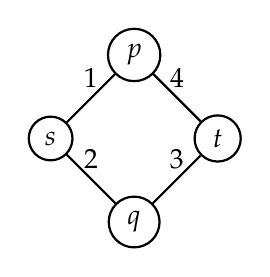
\begin{tikzpicture}[node distance={15mm}, thick, main/.style = {draw, circle}] 
    \node[main] (1) {$s$}; 
    \node[main] (2) [above right of=1] {$p$};
    \node[main] (3) [below right of=1] {$q$}; 
    \node[main] (4) [above right of=3] {$t$};
    \draw (1)--(2) node [midway,above] {1};
    \draw (2)--(4) node [midway,above] {4};
    \draw (1)--(3) node [midway,above] {2};
    \draw (3)--(4) node [midway,above] {3};
\end{tikzpicture} 

(b) Consider the following graph where increasing each edge weight by $k$ does not increase the shortest distance by a factor of k.

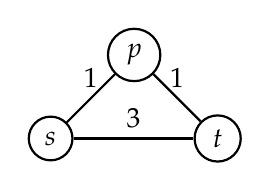
\begin{tikzpicture}[node distance={15mm}, thick, main/.style = {draw, circle}] 
    \node[main] (1) {$s$}; 
    \node[main] (2) [above right of=1] {$p$};
    \node[main] (3) [below right of=2] {$t$};
    \draw (1)--(2) node [midway,above] {1};
    \draw (2)--(3) node [midway,above] {1};
    \draw (1)--(3) node [midway,above] {3};
\end{tikzpicture}
$\rightarrow$
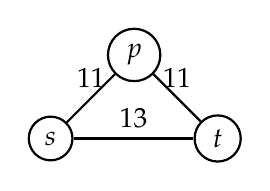
\begin{tikzpicture}[node distance={15mm}, thick, main/.style = {draw, circle}] 
    \node[main] (1) {$s$}; 
    \node[main] (2) [above right of=1] {$p$};
    \node[main] (3) [below right of=2] {$t$};
    \draw (1)--(2) node [midway,above] {11};
    \draw (2)--(3) node [midway,above] {11};
    \draw (1)--(3) node [midway,above] {13};
\end{tikzpicture}

When $k=10$, the shortest path increases from 2 to 13 which is not a factor of $k$. Increasing all edges by k means we favor paths with less edges.

(c) If any edge weight was decreased by $k$, then there are two possibilities. Either edge $e$ was part of our shortest path or it was not. If $e$ was not in shortest path, then our shortest path cost will not decrease at all. If $e$ was in our shortest path, then our shortest path will decrease by $k$. Therefore, decreasing an arbitrary edge by $k$ will decrease our total weight cost by at most $k$.

(d) Consider the following graph where squaring the edge weights changes which nodes are visited in creating a single shortest path.

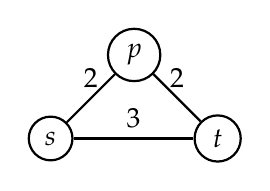
\begin{tikzpicture}[node distance={15mm}, thick, main/.style = {draw, circle}] 
    \node[main] (1) {$s$}; 
    \node[main] (2) [above right of=1] {$p$};
    \node[main] (3) [below right of=2] {$t$};
    \draw (1)--(2) node [midway,above] {2};
    \draw (2)--(3) node [midway,above] {2};
    \draw (1)--(3) node [midway,above] {3};
\end{tikzpicture}
$\rightarrow$
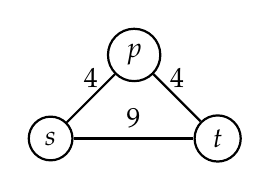
\begin{tikzpicture}[node distance={15mm}, thick, main/.style = {draw, circle}] 
    \node[main] (1) {$s$}; 
    \node[main] (2) [above right of=1] {$p$};
    \node[main] (3) [below right of=2] {$t$};
    \draw (1)--(2) node [midway,above] {4};
    \draw (2)--(3) node [midway,above] {4};
    \draw (1)--(3) node [midway,above] {9};
\end{tikzpicture}

The shortest path is not the same as before with different edge weights, but rather it is in an entirely different path.
\begin{problem}{5}
    Consider a directed, weighted graph $G$ where all edge weights are positive. Propose an efficient method based on Dijkstra's algorithm to find a lowest-cost path from node $s$ to node $t$, given that you may set one edge weight to zero.
\end{problem}
\textit{Answer:} Dijkstra's algorithm is able to give us the distance from a start node to every other node. Given that we know our start node and end node, we can run Dijkstra's twice beginning once with the start node to every other node and once from the end node to every other node after reversing the edge directions in the graph. Let the result from the first Dijkstra's from $s$ be the res[i]. Let the result of the distance from every node to $t$ be stored in reverse[i].

Given arbitary $u,v\in V$, the shortest path from $s$ to $u$ was given by the first run of Dijkstra's and is stored in res[$u$]. Similarly, the shortest path from $v$ to $t$ is stored in reverse[$v$]. Going down the path of $s \rightarrow u \rightarrow v \rightarrow t$, we can find the maximum difference between res[u]+ reverse[v] + e and res[u]+ reverse[v]. When we find  the maximum difference, we know that this is the edge that we can remove that then results in the shortest path. 

We can loop through all nodes that are found in the path, and at each pair of edges, we can do the above check to then find the maximum edge weight that would result in the new shortest path when becoming zero.
\end{document}
